\chapter{A Spatial Model for Rare Binary Events}
\label{chap:three}
\section{Introduction}\label{s:intro}

The goal in binary regression is to relate a latent variable to a response using a link function.
% $g$ so that P$(Y_i=1) = \pi_i= g(\bX_i \bbeta)$, where $\bX_i$ is the vector of covariates for observation $i$, and $\bbeta$ is the $p$-vector of regression coefficients.
Two common examples of binary regression include logistic regression
% with $\pi_i = \frac{ \exp{\bX_i \bbeta} }{1 + \exp{\bX_i \bbeta}}$
and probit regression.
% with $\pi_i = \Phi(\bX_i \bbeta)$ where $\Phi(\cdot)$ represents the standard normal distribution function.
The link functions for logistic and probit regression are symmetric, so they may not be well-suited for asymmetric data.
% In the case that $\xi = 0$, this is the complementary log-log (cloglog) link function.
An asymmetric alternative to these link functions is the complementary log-log (cloglog) link function.
More recently, \citet{Wang2010} introduced the generalized extreme value (GEV) link function for rare binary data.
The GEV link function introduces a new shape parameter to the link function that controls the degree of asymmetry.
The cloglog link is a special case of the GEV link function when the shape parameter is 0.
% where

\hl{Want to make the case in this paragraph that spatial logistic and probit models are not appropriate because asymptotic dependence is 0.}
Spatial logistic and probit models are commonly presented using a hierarchical model \hl{citation}.
In the hierarchical framework, spatial dependence is typically modeled with an underlying latent Gaussian process, and conditioned on this process, observations are independent.
However, if the latent variable is assumed to follow a GEV marginally, then a Gaussian process may not be appropriate to describe the dependence due to the fact that they do not demonstrate asymptotic dependence regardless of the strength of the dependence in the bulk of the data.
As an alternative to the Gaussian process, we propose using a latent max-stable process because it allows for asymptotic dependence \hl{citation}.
Max-stable processes are extremely flexible, but are often challenging to work with because very few finite dimensional representations exist in more than two or three dimensions.


\hl{Paragraph outlining the structure of the paper}

\section{Binary regression using the GEV link}\label{s:rarebinary}

Here, we provide a brief review of the the GEV link of \citet{Wang2010}.
Let $Y_i \in \{0, 1\}, i = 1, \ldots, n$ be a collection of i.i.d. binary responses.
It is assumed that $Y_i = I(z_i > 0)$ where $I(\cdot)$ is an indicator function, $z_i = [1 - \xi \bX_i \bbeta]^{1 / \xi}$ is a latent variable following a GEV$(1, 1, 1)$ distribution, $\bX_i$ be the associated $p$-vector of covariates with first element equal to one for the intercept, and $\bbeta$ is a $p$-vector of regression coefficients.
So, the marginal probability of an event is given by
\begin{align} \label{eq:gevlink}
  \pi_i= 1 - \exp \left( -\frac{ 1 }{ z_i } \right).
\end{align}
Although this link was selected by \citeauthor{Wang2010} based on its ability to handle asymmetry, the GEV distribution is one of the primary distributions used for modeling extremes.
Traditionally, analysis of extreme events is done using block maxima or occurrences over a suitably high threshold.
Because extreme events are rare, it is therefore reasonable to use similar methods when analyzing rare binary data.

\section{Spatial dependence for binary regression}

In many binary regression applications, spatial dependence is handled using a hierarchical model assuming an latent spatial process.
Let $Y(\bs)$ be the observation at spatial location $\bs$ in a spatial domain of interest $\calD \in \calR^2$.
We assume $Y(\bs) = I[Z(\bs) > 0]$ where $Z(\bs)$ is a latent spatial process.
In spatial logistic and probit regression, the latent spatial process is assumed to be a Gaussian process.
A Gaussian process may not be appropriate when describing dependence in the tails of the distribution because it always exhibits asymptotic independence, except in the case of perfect dependence.
Because we use extreme values analysis as the foundation for rare binary analysis, we propose useing a max-stable process to model the latent spatial process

% \subsection{Gaussian process}\label{s:nonrarespatial}

% In this section we present the spatial logistic and probit models.

% In the case that $n$ is large, low-rank predictive process models can be used to ease the computation.

% \subsection{Max-stable process}\label{s:rarebinary}

A max-stable process has generalized extreme value marginal distributions with location $\bX^T(\bs) \bbeta$, scale $\sigma$, and shape $\xi$.
For identifiability purposes we fix $\sigma = 1$.
Although $\bbeta$ and $\xi$ could be permitted to vary across space, we assume that they are constant across $\calD$.

For a finite collection of locations $\bs_1, \ldots, \bs_n,$ denote the vector of observations $\bY = [Y(\bs_1), \ldots, Y(\bs_n)]^T$.
The spatial dependence is determined by the joint distribution of $\bZ = [Z(\bs_1),\ldots, Z(\bs_n)]^T$,
\begin{align}\label{eq:jointCDF}
  G(\bz) = \mbox{P}[Z(\bs_1) < z(\bs_1), \ldots, Z(\bs_n) < z(\bs_n)] = \exp\left\{-\sum_{l=1}^L\left[\sum_{i=1}^n\left(\frac{w_{l}(\bs_i)}{z(\bs_i)}\right)^{1/\alpha}\right]^{\alpha}\right\},
\end{align}
where $w_{l}(\bs_i)$ are a set of $L$ weights that determine the spatial dependence structure, and $\alpha\in(0,1)$ determines the strength of dependence, with $\alpha$ near zero giving strong dependence and $\alpha=1$ giving joint independence.
This is a special case of the multivariate GEV distribution with asymmetric Laplace dependence function \citep{Tawn1990}.
The weights $w_{l}(\bs_i)$ in (\ref{eq:jointCDF}) vary smoothly across space to induce spatial dependence.
Many weight functions are possible, but the weights must be constrained so that $\sum_{l=1}^L w_{l}(\bs_i)=1$ for all $i=1,\ldots,n$ to preserve the marginal GEV distribution.
For example, \cite{Reich2012} take the weights to be scaled Gaussian kernels with knots $\bv_l$,
\begin{align}\label{w}
   w_{l}(\bs_i) = \frac{\exp\left[-0.5\left(||\bs_i-\bv_l||/\rho\right)^2\right]}
                 {\sum_{j=1}^L\exp\left[-0.5\left(||\bs_i-\bv_j||/\rho\right)^2\right]}.
\end{align}
The kernel bandwidth $\rho>0$ determines the spatial range of the dependence, with large $\rho$ giving long-range dependence and vice versa.

One nice feature to this representation for the max-stable process is that the lower-dimensional marginal distributions also follow a multivariate extreme value distribution.
More importantly, at a single site $i$, the marginal distribution gives \mbox{$P[Y(\bs_i) = 1] = 1 - \exp\left[ -\frac{ 1 }{ z(\bs_i)} \right]$} which is the same as the marginal distribution given by \citet{Wang2010}.

The joint likelihood of $Y$ is computationally challenging to obtain.
Therefore, to incorporate spatial dependence into the model, we consider the hierarchical max-stable process of \citet{Reich2012}.
Consider a set of $A_1, \ldots, A_l \iid \text{PS}(\alpha)$ random effects associated with spatial knots $\bv_1, \ldots, \bv_L$.
The hierarchical model is given by
\begin{align} \label{eq:hiermodel}
  Z(\bs) | A_l, \ldots, A_l &\indep \text{GEV}[\theta(\bs), \alpha \theta(\bs), \alpha] \\
  A_l &\iid \text{PS}(\alpha) \nonumber
\end{align}
where $\theta(\bs) = \left[\sum_{l = 1}^L A_l w_l (\bs)^{1 / \alpha} \right]^\alpha$.

% \subsubsection{Weight functions}\label{s:weights}


\section{Joint distribution}\label{s:multivariate}

In section \ref{s:bivariate}, we give an exact expression in the case where there are only two spatial locations which is useful for constructing a pairwise composite likelihood and studying spatial dependence.
For more than two locations, we are also able to compute the exact likelihood when the number of locations is large but the number of events is small, as might be expected for very rare events (see Appendix \ref{a:likelihoodderivation}).

\subsection{Bivariate distribution}\label{s:bivariate}
Then in a bivariate setting, the probability mass function as a function of $\alpha$ is
\begin{adjustwidth}{-0.25in}{}
{\footnotesize
\begin{align} \label{biv}
  \text{P}[Y(\bs_i), Y(\bs_j)] = \left\{ \begin{array}{ll}
    \exp \left\{ - \sum_{ l = 1 }^{ L } \left[ \left( \frac{ w_{ l }(\bs_i) }{ z(\bs_i) } \right)^{1/\alpha} + \left( \frac{ w_{l }(\bs_j)}{z(\bs_j)} \right)^{1/\alpha} \right]^{\alpha} \right\} &Y(\bs_i) = 0, Y(\bs_j) = 0\\
    \frac{ 1 }{z(\bs_i)} - \exp \left\{ - \sum_{ l = 1 }^{ L } \left[ \left( \frac{ w_{ l }(\bs_i) }{ z(\bs_i) } \right)^{1/\alpha} + \left( \frac{ w_{l }(\bs_j)}{z(\bs_j)} \right)^{1/\alpha} \right]^{\alpha} \right\} &Y(\bs_i) = 1, Y(\bs_j) = 0 \\
    1 - \exp\left\{ - \frac{ 1 }{ z(\bs_i) } \right\} - \exp \left\{ - \frac{ 1 }{z(\bs_j)} \right\} + \exp \left\{ - \sum_{ l = 1 }^{ L } \left[ \left( \frac{ w_{ l }(\bs_i) }{ z(\bs_i) } \right)^{1/\alpha} + \left( \frac{ w_{l }(\bs_j)}{z(\bs_j)} \right)^{1/\alpha} \right]^{\alpha} \right\} &Y(\bs_i) = 1, Y(\bs_j) = 1
  \end{array} \right.
\end{align}
}
\end{adjustwidth}

\section{Quantifying spatial dependence}
\hl{I still need to incorporate Brian's suggestions here}
In the literature on extremes, one common metric to describe the bivariate dependence is the $\chi$ statistic of \citet{Coles1999}.
The $\chi$ statistic between two observations $z_1$ and $z_2$ is given by
\begin{align}
  \chi(\bs_1, \bs_2) = \lim_{c \rightarrow \infty} = P(Z_1 > c | Z_2 > c).
\end{align}
However, in this latent variable approach, $\lim_{c \rightarrow \infty}$ may not be the most reasonable metric because the observed data are a series of zeros and ones.
Therefore, we chose the $\kappa$ statistic of \citet{Cohen1960} defined by
\begin{align}
  \kappa = \frac{P(A) - P(E)}{1 - P(E)}
\end{align}
where $P(A)$ is the joint probability of agreement and $P(E)$ is the joint probability of agreement under an assumption of independence.
We believe this measure of dependence to be reasonable because,
\begin{align}
  \lim_{\beta_0 \rightarrow \infty} \kappa(h) = \chi(h) = 2 - \vartheta(\bs_i, \bs_j)
\end{align}
where $\beta_0$ is the intercept from $\bX^T\bbeta$ and $\vartheta (\bs_i, \bs_j) = \sum_{ l = 1 }^{ L } \left[ w_{l}(\bs_i)^{ 1/\alpha } +  w_{ l}(\bs_j)^{ 1/\alpha } \right]^\alpha$ is the pairwise extremal coefficient given by \citet{Reich2012} (see Appendix \ref{a:chi}).
In the case of complete dependence, $\kappa = 1$, and in the case of complete independence, $\kappa = 0$.

\section{Computation}\label{s:comp}
For small $K$ we can evaluate the likelihood directly.
When $K$ is large, we use MCMC methods with the random effects model to explore the posterior distribution.
This is possible because the expression for the joint density, conditional on $A_1, \ldots, A_L$, is given by
\begin{align}
  P[Y(\bs_1)=y(\bs_1),\ldots,Y(\bs_n)=y(\bs_n)] = \prod_{ i = 1 }^{ n } \pi(\bs_i)^{ 1 - Y_i } [1 - \pi(\bs_i)]^{ Y_i }.
\end{align}
where
\begin{align}
  \pi(\bs_i) = \exp \left\{ -\sum_{ l = 1 }^{L} A_l \left( \frac{ w_{l}(\bs_i) }{ z(\bs_i) } \right)^{ 1/\alpha} \right\}.
\end{align}

The model parameters and random effects are updated using a combination of Metropolis Hastings (MH) and Hamiltonian Monte Carlo (HMC) update steps.
To overcome challenges with evaluating the positive stable density, we follow \citet{Reich2012} and incorporate the auxiliary variable technique of \citet{Stephenson2009}.


\section{Simulation study}\label{s:sim}

For our simulation study, we generate $n_m = 50$ datasets under 6 different settings to explore the impact of sample size and misspecification of link function.
We generate data assuming three possible types of underlying process.
For each process, we consider two sample sizes $n_s = 650$ and $n_s = 1300$.

The first of these processes is a max-stable process that uses the GEV link described in \ref{eq:hiermodel} with knots on a $21 \times 21$ grid on $[0, 1] \times [0, 1]$.
For this process, we set $\alpha = 0.3$, $\rho = 0.025$, $\xi = 0$ for idenfiability purposes, and $\beta_0$ is set for each dataset to give $5\%$ rarity.
We then set $Y(\bs) = I[z(\bs) > 0]$ where $I[\cdot]$ is an indicator function.

For the second process, we generate a latent variable from a spatial Gaussian process with a mean of $\text{logit}(0.05) \approx -2.9444$ and an exponential covariance given by
\begin{align}
  \text{cov}(\bs_1, \bs_2) = \tau_\text{Gau}^2 * \exp\left\{- \frac{||\bs_1 - \bs_2||}{\rho_\text{Gau}}\right\}
\end{align}
where $\tau_\text{Gau} = 7$ and $\rho_\text{Gau} = 0.10$.
The mean of the Gaussian process is set to give approximately $5\%$ rarity.
Finally, we generate $Y(\bs) \ind \text{Bern}[\pi(\bs)]$
where $\pi(\bs) = \exp\left\{ \frac{z(\bs)}{1 + z(\bs)} \right\}$

For the third process, we generate data using a hotspot method.
For this process, we first generate hotspots throughout the space, and then set the probability of occurrence to be higher when a site is within a circle of radius $\rho = 0.05$ from a hotspot location.
More specifically, generate $K \sim \text{Poisson}(9)$ hotspot locations, $\bv^*_1, \ldots, \bv^*_K$, from a uniform distribution over $[0, 1] \times [0, 1]$.
If $||\bs_i - \bv^*_k|| < 0.05$ for any $k$, then $\pi(\bs_i) = 0.70$ otherwise, $\pi(\bs_i) = 0.01$.
We then generate $Y(\bs_i) \ind \text{Bern}[\pi(\bs_i)]$.

For each dataset, we fit the model using three different methods, spatial logistic regression, spatial probit regression, and the proposed spatial GEV method.

\subsection{Spatial logistic and probit methods}
Because logistic and probit methods represent two of the more common spatial techniques for binary data, we chose to compare our method to them.
One way these methods differ from our proposed method is that they assume the underlying process is Gaussian.
In this case, we assume that $Z(\bs)$ follows a Gaussian process with mean $\bX(s)^T \bbeta$ and exponential covariance function.
The marginal distributions are given by
\begin{align}
  P(Y = 1) = \left\{ \begin{array}{ll}
    \frac{\exp[\bX^T \bbeta + \bW \balpha]}{1 + \exp[\bX^T \bbeta + \bW \balpha]}, \qquad &\text{logistic}\\
    \phi(\bX^T \bbeta + \bW \balpha), \qquad &\text{probit}
  \end{array}\right.
\end{align}
where $\balpha$ are Gaussian random effects at the knot locations, and the $\bW$ are basis functions to recreate the Gaussian process at all sites.

\subsection{Cross validation}\label{s:modelselect}
For each dataset, we fit the model using 500 of the observations as a training set, and the remaining observations are used as a validation set to assess the model's predictive power.
Because our goal is to predict a the occurrence of an event, we use Brier scores to compare the models \citep{Gneiting2007}.
The Brier score for predicting an occurrence at site $\bs$ is given by $\{I[Y(\bs)=1] - P[Y(\bs)=1]\}^2$ where $I[Y(\bs) = 1]$ is an indicator function indicating that an event occurred at site $\bs$, and $P[Y(\bs) = 1]$ is obtained by taking the median of the posterior distribution.
We average the Brier scores over all test sites, and a lower score indicates a better fit.

We also consider the receiver operating characteristic (ROC) curve and look at the area under the curve (AUC) for the different methods and settings.
AUC is commonly used as a metric to determine how well a model can classify data.
When AUC = 1, the model perfectly classifies all observations in the test set, and when AUC = 0, the model misclassifies all observations in the test set.
AUC is computed using the \texttt{roc} function in the \texttt{pROC} package of \texttt{R} using the median of the posterior predictive distribution at the testing locations.
We then average AUCs across all datasets for each method and setting to obtain a single AUC for each combination of method and setting.

\subsection{Results}
Table \ref{tbl:simbsresults} gives the Brier score relative to the Brier score for the spatial logistic method calculated as
\begin{align}
  \text{BS}_{\text{rel}} = \frac{\text{BS}_{\text{method}}}{\text{BS}_{\text{logistic}}}.
\end{align}
Table \ref{tbl:simaucresults} gives the AUC relative to the AUC for the spatial logistic method calculated in similarly to the relative Brier score.

\begin{table}
  \caption{Relative Brier scores for GEV and Probit methods}
  \label{tbl:simbsresults}
  \centering
  \begin{tabular}{r|ll}
    \cline{2-3}
              & GEV    & Probit\\
    \hline
    Setting 1 & 0.9047 & 0.9754\\
    Setting 2 & 0.7885 & 0.9804\\
    Setting 3 & 1.0275 & 1.0018\\
    Setting 4 & 1.0264 & 1.0089\\
    Setting 5 & 1.0458 & 0.9963\\
    Setting 6 & 1.0565 & 0.9945\\
    \hline
  \end{tabular}
\end{table}

\begin{table}
  \caption{Relative AUC for GEV and Probit methods}
  \label{tbl:simaucresults}
  \centering
  \begin{tabular}{r|lll}
    \cline{2-4}
              & GEV    & Probit & Logit\\
    \hline
    Setting 1 & 0.8998 & 0.8973 & 0.8897\\
    Setting 2 & 0.9458 & 0.9399 & 0.9356\\
    Setting 3 & 0.7288 & 0.7371 & 0.7157\\
    Setting 4 & 0.7906 & 0.8056 & 0.8115\\
    Setting 5 & 0.8426 & 0.8458 & 0.8388\\
    Setting 6 & 0.8756 & 0.8686 & 0.8765\\
    \hline
  \end{tabular}
\end{table}

We analyzed the results for this simulation study using a Friedman test at $\alpha = 0.05$ to see if at least one method had a significantly different Brier score or AUC.
For any setting that yielded a significant p-value, we conducted a Wilcoxon-Nemenyi-McDonald-Thompson test to see which of the methods had different results.
The full results for the Wilcoxon-Nemenyi-McDonald-Thompson tests are given in Appendix \ref{a:pdiffs}.
For all settings, we find significant results for the Friedman test comparing the Brier scores for the methods.
Specifcally, we see a statistically significant reduction in Brier score using the GEV compared to logit for settings 1 and 2 and compared to probit for setting 2.
However, in the other settings, the logit and probit methods tend to perform better than the GEV method.

The results using AUC are much less conclusive with only settings 1 and 4 demonstrating significant differences between the methods at $\alpha = 0.05$.
As with the Brier scores, the GEV method shows a statistically significant increase in AUC over the logit method for setting 1, and for setting 4, the both the probit and logit methods show a statistically significant improvement in AUC over the GEV method.

% Figures \ref{fig:post-med-2} and \ref{fig:post-med-3} show the posterior median of $P(Y =1)$ for settings 2 and 3 respectively of a simulated dataset.
% As you can see on the figures, the both the spatial probit and logistic models oversmooth $P(Y = 1)$, whereas the spatial GEV method is able to capture small pockets of spatial dependence.
% Plots for the medians of settings 1 and 4 look similar, so they are not included here.

% \begin{figure}
%   % this figure comes from markdown/sim-hmc/predict-maps.R
%   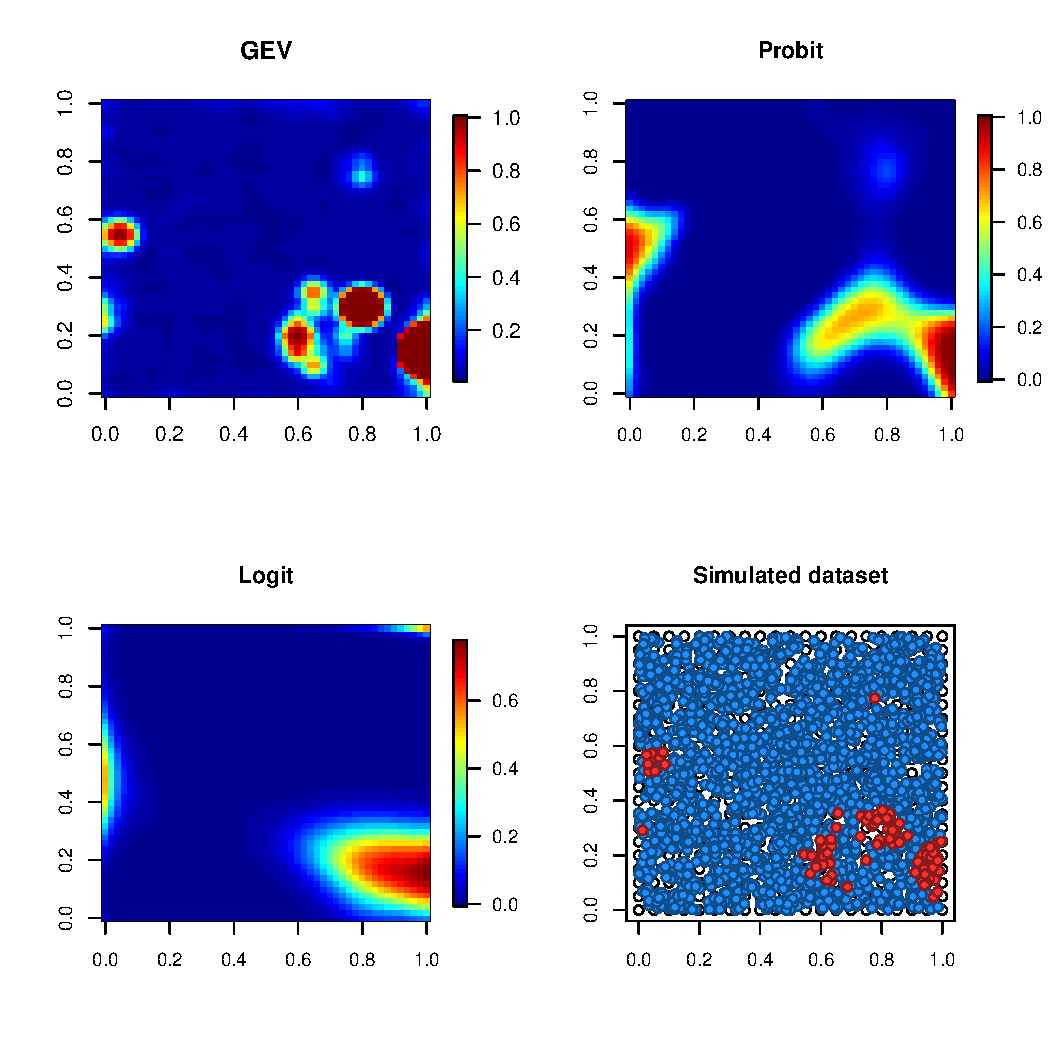
\includegraphics[width=\linewidth]{plots/post-med-2.pdf}
%   \caption{Posterior median $P(Y = 1)$ for spatial GEV, probit, and logistic regression for setting 2.}
%   \label{fig:post-med-2}
% \end{figure}

% \begin{figure}
%   % this figure comes from markdown/sim-hmc/predict-maps.R
%   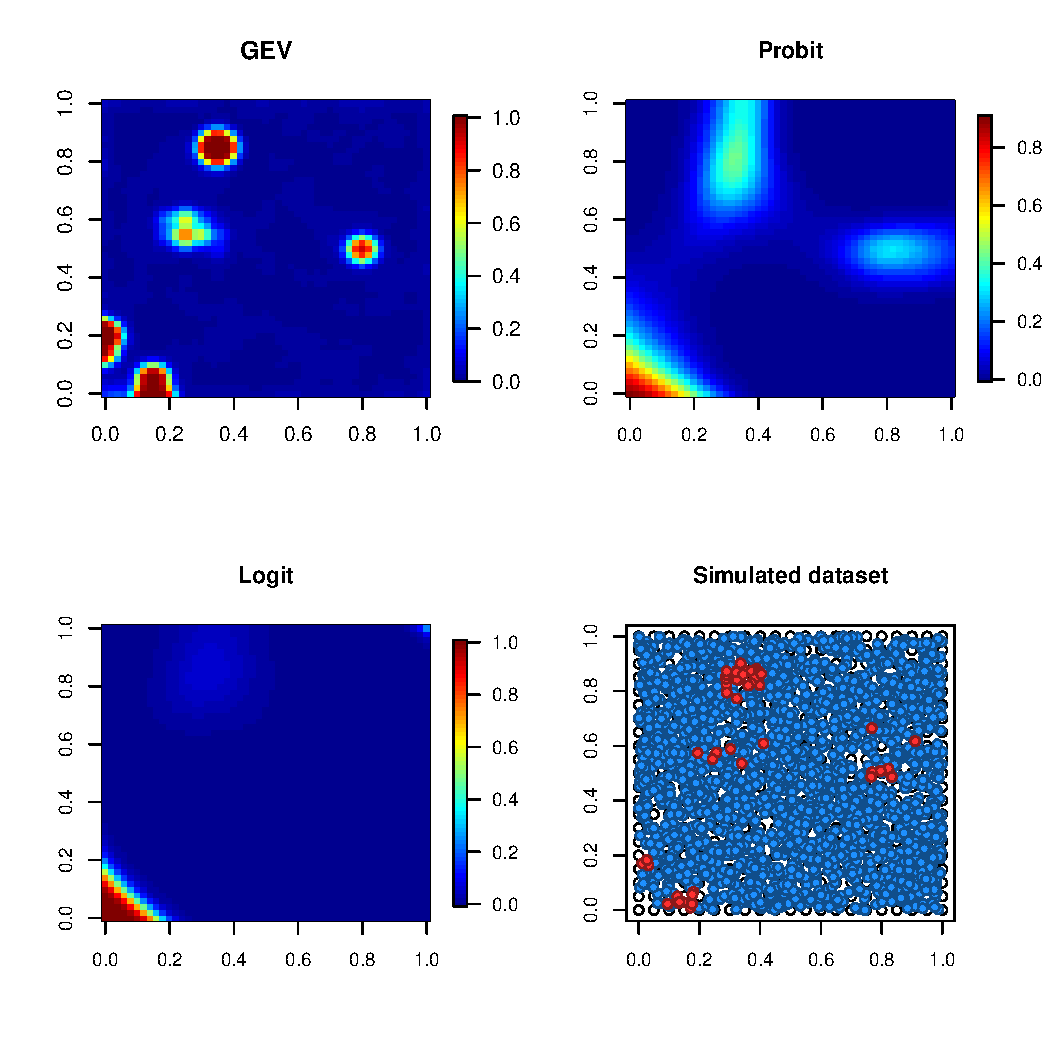
\includegraphics[width=\linewidth]{plots/post-med-3.pdf}
%   \caption{Posterior median $P(Y = 1)$ for spatial GEV, probit, and logistic regression for setting 3.}
%   \label{fig:post-med-3}
% \end{figure}

\section{Data analysis}\label{s:analysis}
For the data analysis, we consider data from the eBirds dataset, a citizen-based observation network of bird sitings in the United States \citep{Sullivan2009}.
The data are publicly available from {\tt http://ebird.org}.
We use data from 2002, and focus on 10 different species.
Figure \ref{fig:data2002} shows the sighting data for cattle egrets and vesper sparrows

\begin{figure}
  \centering
  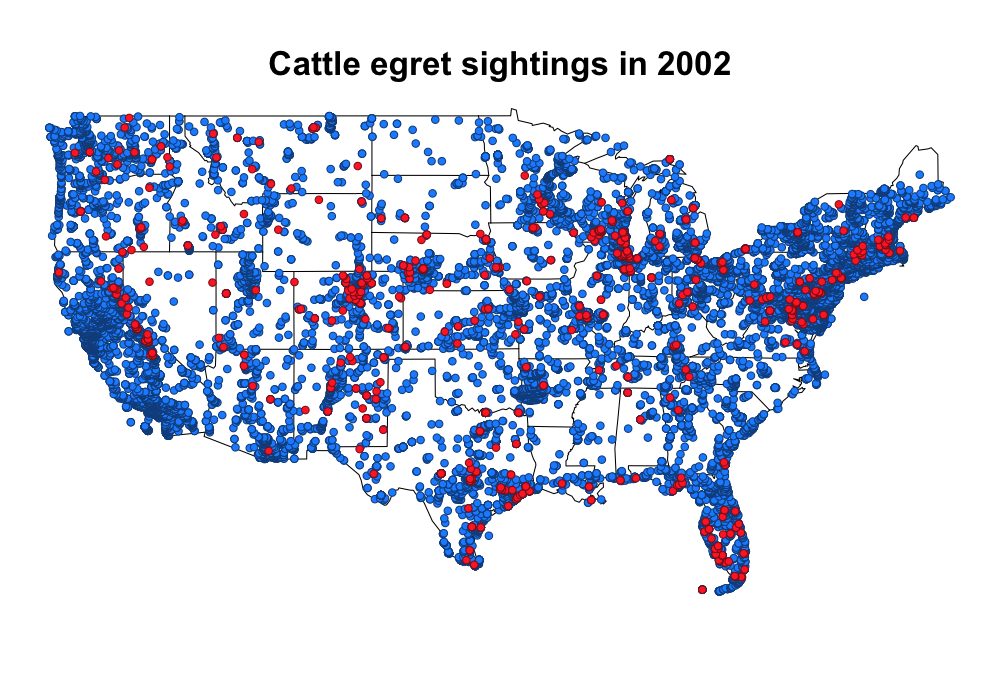
\includegraphics[width=0.47\linewidth]{plots/cattle_egret.png}
  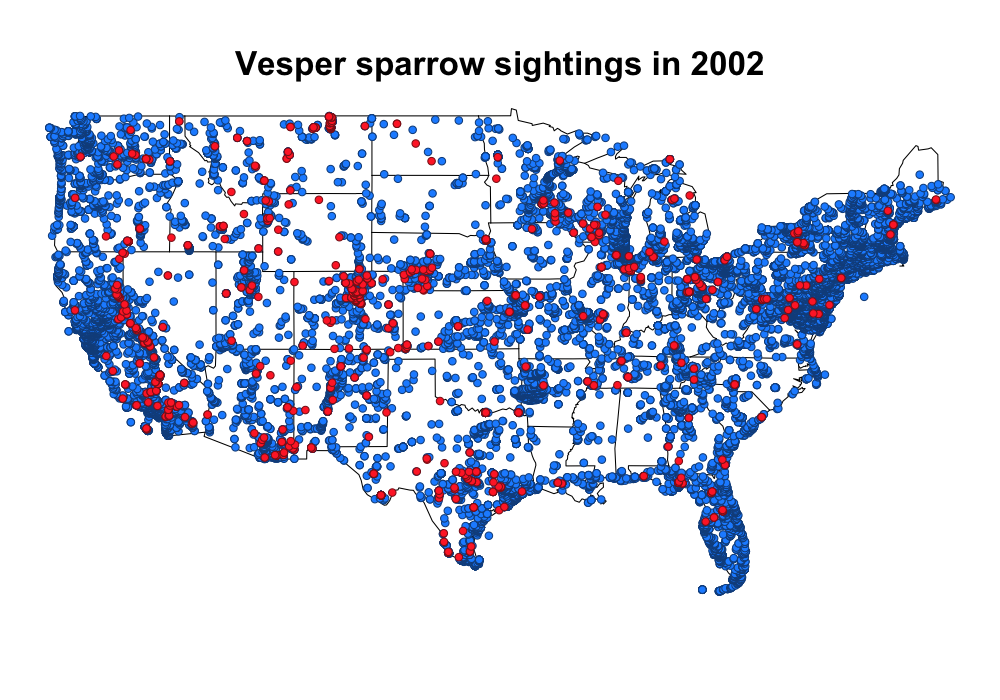
\includegraphics[width=0.47\linewidth]{plots/vesper_sparrow.png}
  \caption{Reported sighting for Cattle egret (left) and Vesper sparrow (right) in 2002}
  \label{fig:data2002}
\end{figure}b

\section{Conclusions}\label{s:con}

\section*{Acknowledgments}

\appendix
\section{Appendices}

\subsection{Derivation of the likelihood} \label{a:likelihoodderivation}
We use the hierarchical max-stable spatial model given by \citet{Reich2012}. If at each margin, $Z_i \sim $ GEV$(1,1,1)$, then $Z_i | \theta_i \indep $ GEV$(\theta, \alpha \theta, \alpha)$. We reorder the data such that $Y_1=\ldots=Y_K=1$, and $Y_{K+1} = \ldots = Y_n = 0$. Then the joint likelihood conditional on the random effect $\theta$ is

\begin{align} \label{joint_cond}
  P(Y_1=y_1,\ldots,Y_n=y_n) =& \prod_{ i \le K } \left\{ 1 - \exp \left[ - \left( \frac{ \theta_i }{ z_i } \right)^{ 1/\alpha} \right] \right \} \prod_{ i > K } \exp \left[ -\left( \frac{ \theta_i }{ z_i } \right)^{1/\alpha} \right] \nonumber \\[0.5em]
    =& \exp \left[ -\sum_{ i = K+1}^{ n }\left( \frac{ \theta_i }{ z_i } \right)^{1/\alpha} \right] - \exp \left[ -\sum_{ i = K+1}^{ n }\left( \frac{ \theta_i }{ z_i } \right)^{1/\alpha} \right] \sum_{ i = 1}^{K} \exp\left[ -\left( \frac{ \theta_i }{ z_i } \right)^{ 1/\alpha} \right] \nonumber\\
    &  + \exp \left[ -\sum_{ i = K+1}^{ n }\left( \frac{ \theta_i }{ z_i } \right)^{1/\alpha} \right] \sum_{ 1 < i < j \le K } \left\{ \exp \left[ - \left( \frac{ \theta_i }{ z_i } \right)^{ 1/\alpha} - \left( \frac{ \theta_j }{ z_j } \right)^{ 1/\alpha } \right] \right \} \nonumber \\[0.5em]
    & + \cdots + (-1)^K \exp\left[ - \sum_{ i = 1 }^{ n }\left( \frac{ \theta_i }{ z_i } \right)^{ 1/\alpha} \right]
\end{align}

Finally marginalizing over the random effect, we obtain

\begin{align} \label{joint}
    P(Y_1=y_1,\ldots,Y_n=y_n) =&\int G(\bz | \bA) p( \bA | \alpha) d\bA. \nonumber\\[0.5em]
      =& \int \exp \left[ -\sum_{ i = K+1}^{ n }\left( \frac{ \theta_i }{ z_i } \right)^{1/\alpha} \right] - \exp \left[ -\sum_{ i = K+1}^{ n }\left( \frac{ \theta_i }{ z_i } \right)^{1/\alpha} \right] \sum_{ i = 1}^{K} \exp\left[ -\left( \frac{ \theta_i }{ z_i } \right)^{ 1/\alpha} \right] \nonumber\\
    &  + \exp \left[ -\sum_{ i = K+1}^{ n }\left( \frac{ \theta_i }{ z_i } \right)^{1/\alpha} \right] \sum_{ 1 < i < j \le K } \left\{ \exp \left[ - \left( \frac{ \theta_i }{ z_i } \right)^{ 1/\alpha} - \left( \frac{ \theta_j }{ z_j } \right)^{ 1/\alpha } \right] \right \} \nonumber \\[0.5em]
    & + \cdots + (-1)^K \exp\left[ - \sum_{ i = 1 }^{ n }\left( \frac{ \theta_i }{ z_i } \right)^{ 1/\alpha} \right] p( \bA | \alpha) d\bA.
\end{align}

Consider the first term in the summation,

\begin{align}
  \int \exp \left\{ -\sum_{ i = K+1}^{ n }\left( \frac{ \theta_i }{ z_i } \right)^{1/\alpha} \right\} p( \bA | \alpha) d\bA &= \int \exp \left\{ - \sum_{ i = K + 1 }^n \left( \frac{ \left[ \sum_{ l = 1 }^L  A_l w_{l}(\bs_i)^{1/\alpha} \right)^\alpha }{ z_i} \right]^{ 1/\alpha } \right \} p( \bA | \alpha) d\bA \nonumber \\[0.5em]
   &= \int \exp \left\{ -\sum_{ i = K + 1}^n \sum_{ l = 1}^L A_l \left( \frac{ w_l (\bs_i) }{ z_i } \right)^{1/\alpha} \right \} p( \bA | \alpha) d\bA \nonumber \\[0.5em]
   &=\exp\left\{-\sum_{ l = 1}^L \left[ \sum_{ i = K + 1 }^n \left( \frac{ w_l(\bs_i)}{ z_i} \right)^{1/\alpha} \right]^\alpha \right\}.
\end{align}

The remaining terms in equation (\ref{joint}) are straightforward to obtain, and after integrating out the random effect, the joint density for $K = 0, 1, 2$ is given by
\begin{align}\label{pmf}
  P(Y_1=y_1,\ldots,Y_n=y_n) =  \left\{
    \begin{array}{ll}
      G(\bz) & K=0 \\
      G(\bz_{(1)})-G(\bz) & K=1 \\
      G(\bz_{(12)})-G(\bz_{(1)})-G(\bz_{(2)})+G(\bz) & K=2
    \end{array}
  \right.
\end{align}
where
\begin{align*}
  G[\bz_{(1)}] &= P[Z(\bs_2)<z(\bs_2),\ldots,Z(\bs_n)<z(\bs_n)] \\
  G[\bz_{(2)}] &= P[Z(\bs_1)<z(\bs_1),Z(\bs_3)<z(\bs_3),\ldots,Z(\bs_n)<z(\bs_n)]\\
  G[\bz_{(12)}] &= P[Z(\bs_3)<z(\bs_3),\ldots,Z(\bs_n)<z(\bs_n)].
\end{align*}
Similar expressions can be derived for all $K$, but become cumbersome for large $K$.

\subsection{Derivation of the $\chi$ statistic}\label{a:chi}
\begin{align} \label{chi}
  \chi &= \lim_{p \rightarrow 0 }\text{P}(Y_i = 1|Y_j = 1)\nonumber \\
   &= \lim_{p \rightarrow \infty }\frac{ p + p - \left( 1 - \exp \left \{ - \sum_{ l = 1 }^{ L } \left[ \left( -\log(1-p) w_{l}(\bs_i) \right)^{ 1/\alpha } + \left( -\log(1 - p) w_{ l}(\bs_j) \right)^{ 1/\alpha } \right]^{\alpha} \right \} \right) }{ p } \nonumber \\[0.5em]
  &= \lim_{p \rightarrow 0 } \frac{ 2p - \left( 1 - \exp \left \{ \log(1-p) \sum_{ l = 1 }^{ L } \left[  w_{l}(\bs_i) ^{ 1/\alpha } +  w_{ l}(\bs_j) ^{ 1/\alpha } \right]^{\alpha} \right \} \right) }{ p } \nonumber \\[0.5em]
  &= \lim_{p \rightarrow 0 } \frac{ 2p - \left( 1 - (1-p)^{ \sum_{ l = 1 }^{ L } \left[ \left( w_{l}(\bs_i) \right)^{ 1/\alpha } + \left( w_{ l}(\bs_j) \right)^{ 1/\alpha } \right]^\alpha } \right) }{ p } \nonumber \\[0.5em]
  &=\lim_{p \rightarrow 0 } 2 -\sum_{ l = 1 }^{ L } \left[ w_{l}(\bs_i) ^{ 1/\alpha } +  w_{ l} (\bs_j)^{ 1/\alpha } \right]^\alpha ( 1 - p)^{ -1 + \sum_{ l = 1 }^{ L } \left[  w_{l}(\bs_i) ^{ 1/\alpha } +  w_{ l}(\bs_j)^{ 1/\alpha } \right]^\alpha } \nonumber \\[0.5em]
  &= 2 -  \sum_{ l = 1 }^{ L } \left[ w_{l}(\bs_i)^{ 1/\alpha } +  w_{ l}(\bs_j) ^{ 1/\alpha } \right]^\alpha.
\end{align}